\documentclass[uct_visualisation_thesis.tex]{subfiles}

% ------------------- 1. SŁOWNICZEK ---------------------
\chapter{Wykaz najważniejszych oznaczeń i skrótów}
\begin{itemize}
	\item \textbf{MCTS} (Monte Carlo Tree Search) - heurystyka podejmowania decyzji w pewnych zadaniach sztucznej inteligencji, np. ruchów w grach. Najczęściej MCTS opiera się na wariancie metody UCT.
	\item \textbf{UCT} (Upper Confidence Bound Applied to Trees) - algorytm przeszukujący drzewo stanów rozgrywki w poszukiwaniu najbardziej opłacalnych ruchów. Algorytm stara się zachować równowagę między eksploatacją ruchów po ruchach o wysokiej średniej wygranej a eksploracją tych mało sprawdzonych.
	\item \textbf{Podstawowa wizualizacja} - możliwość wyświetlenia całego drzewa stanów. W podstawowej wizualizacji wygląd wierzchołków i krawędzi jest nieistotny.
	\item \textbf{Zaawansowana wizualizacja} - podstawowa wizualizacja wzbogacona o możliwość analizowania statystyk poszczególnych wierzchołków. Kolor wierzchołków będzie reprezentował aktualnego gracza, a kolor krawędzi częstość odwiedzin danego węzła. Możliwe powinno być też przewijanie, przybliżanie oraz oddalanie podglądu drzewa.
	\item \textbf{CSV} - plik w formacie .csv (ang. \textit{comma-separated values}) służący do przechowywania danych w plikach tekstowych, gdzie separatorem jest przecinek.
\end{itemize}

% ------------------- 2. WSTĘP ---------------------
\chapter{Wstęp i cel pracy}
\section{Cel biznesowy}
Algorytm UCT, będący usprawnieniem MCTS, jest powszechnie stosowanym algorytmem w sztucznej inteligencji. Jest metodą analizującą obiecujące ruchy na podstawie generowanego drzewa, która równoważy eksploatację najbardziej korzystnych z eksploracją mniej korzystnych decyzji. Każdemu wierzchołkowi drzewa odpowiada pewien stan rozgrywki, z którego algorytm rozgrywa losowe symulacje, rozszerzając potem drzewo o kolejne możliwe stany. Sposób, w jaki rozrasta się opisywane drzewo, jest kluczowy dla podejmowania przez algorytm jak najlepszych decyzji.\\

Celem projektu jest stworzenie aplikacji pozwalającej na wizualizację drzew algorytmu UCT. Aplikacja będzie pozwalała na wizualizowanie drzew generowanych podczas rozgrywania dwóch przykładowych gier (pozwalając przetestować rozwiązanie). Aplikacja powinna pozwalać na wizualizację drzew, ich sekwencji i róznic między kolejnymi drzewami w sekwencji. Powinna być możliwość płynnego przybliżania/oddalania i przewijania wizualizacji oraz zapisu aktualnego stanu do pliku graficznego - wszystko, aby klient mógł wygodnie korzystać z naszego programu. Taki produkt pozwoliłby zrozumieć klientowi ideę i sposób działania algorytmu UCT.
\section{Założenia projektowe}
\subsection{Założenia funkcjonalne}
Użytkownik korzystający z naszej aplikacji będzie mógł wybrać jedną z dwóch gier deterministycznych, a do wyboru będzie miał trzy tryby rozgrywki:
\begin{enumerate}
	\item Gracz vs PC -- użytkownik będzie decydował o swoich posunięciach i zmierzy się on z zaimplementowanym algorytmem,
	\item PC vs PC -- użytkownik będzie świadkiem symulacji algorytmu, który rozgrywa partię z samym sobą,
	\item Gracz vs Gracz -- rozgrywka dwóch graczy, bez wizualizacji.\\
\end{enumerate}
Zanim jednak przejdzie do rozgrywki, będzie on miał możliwość ustawienia parametrów algorytmu, tj. liczbę iteracji podczas tworzenia drzewa, czy też maksymalny czas na ruch przeciwnika.
Druga opcja, którą będzie dysponować użytkownik, to możliwość wczytania drzewa w formacie zarówno binarnym jak i CSV.
a następnie możliwość jego dogłębnej analizy. Będzie on mógł wyświetlać informacje na temat wybranego węzła, a także przybliżać i oddalać całą wygenerowaną strukturę. Podczas samej rozgrywki, po wykonanym ruchu przeciwnika gracz będzie mógł analizować drzewo w sposób opisany powyżej, a także wyeksportować je. Będzie też miał możliwość zapisania go w wyżej wymienionych formatach, a także w formacie rastrowym. Użytkownik będzie mógł oglądać animację rozrostu drzewa. Powyższe rzeczy dotyczą trybów gry z udziałem algorytmu i każdej z gier. \\\\
Diagram przypadków użycia, który ilustruje przedstawione możliwości, znajduje się na rysunku \ref{rys:usecase}.
\begin{figure}[h!]
	\centering
	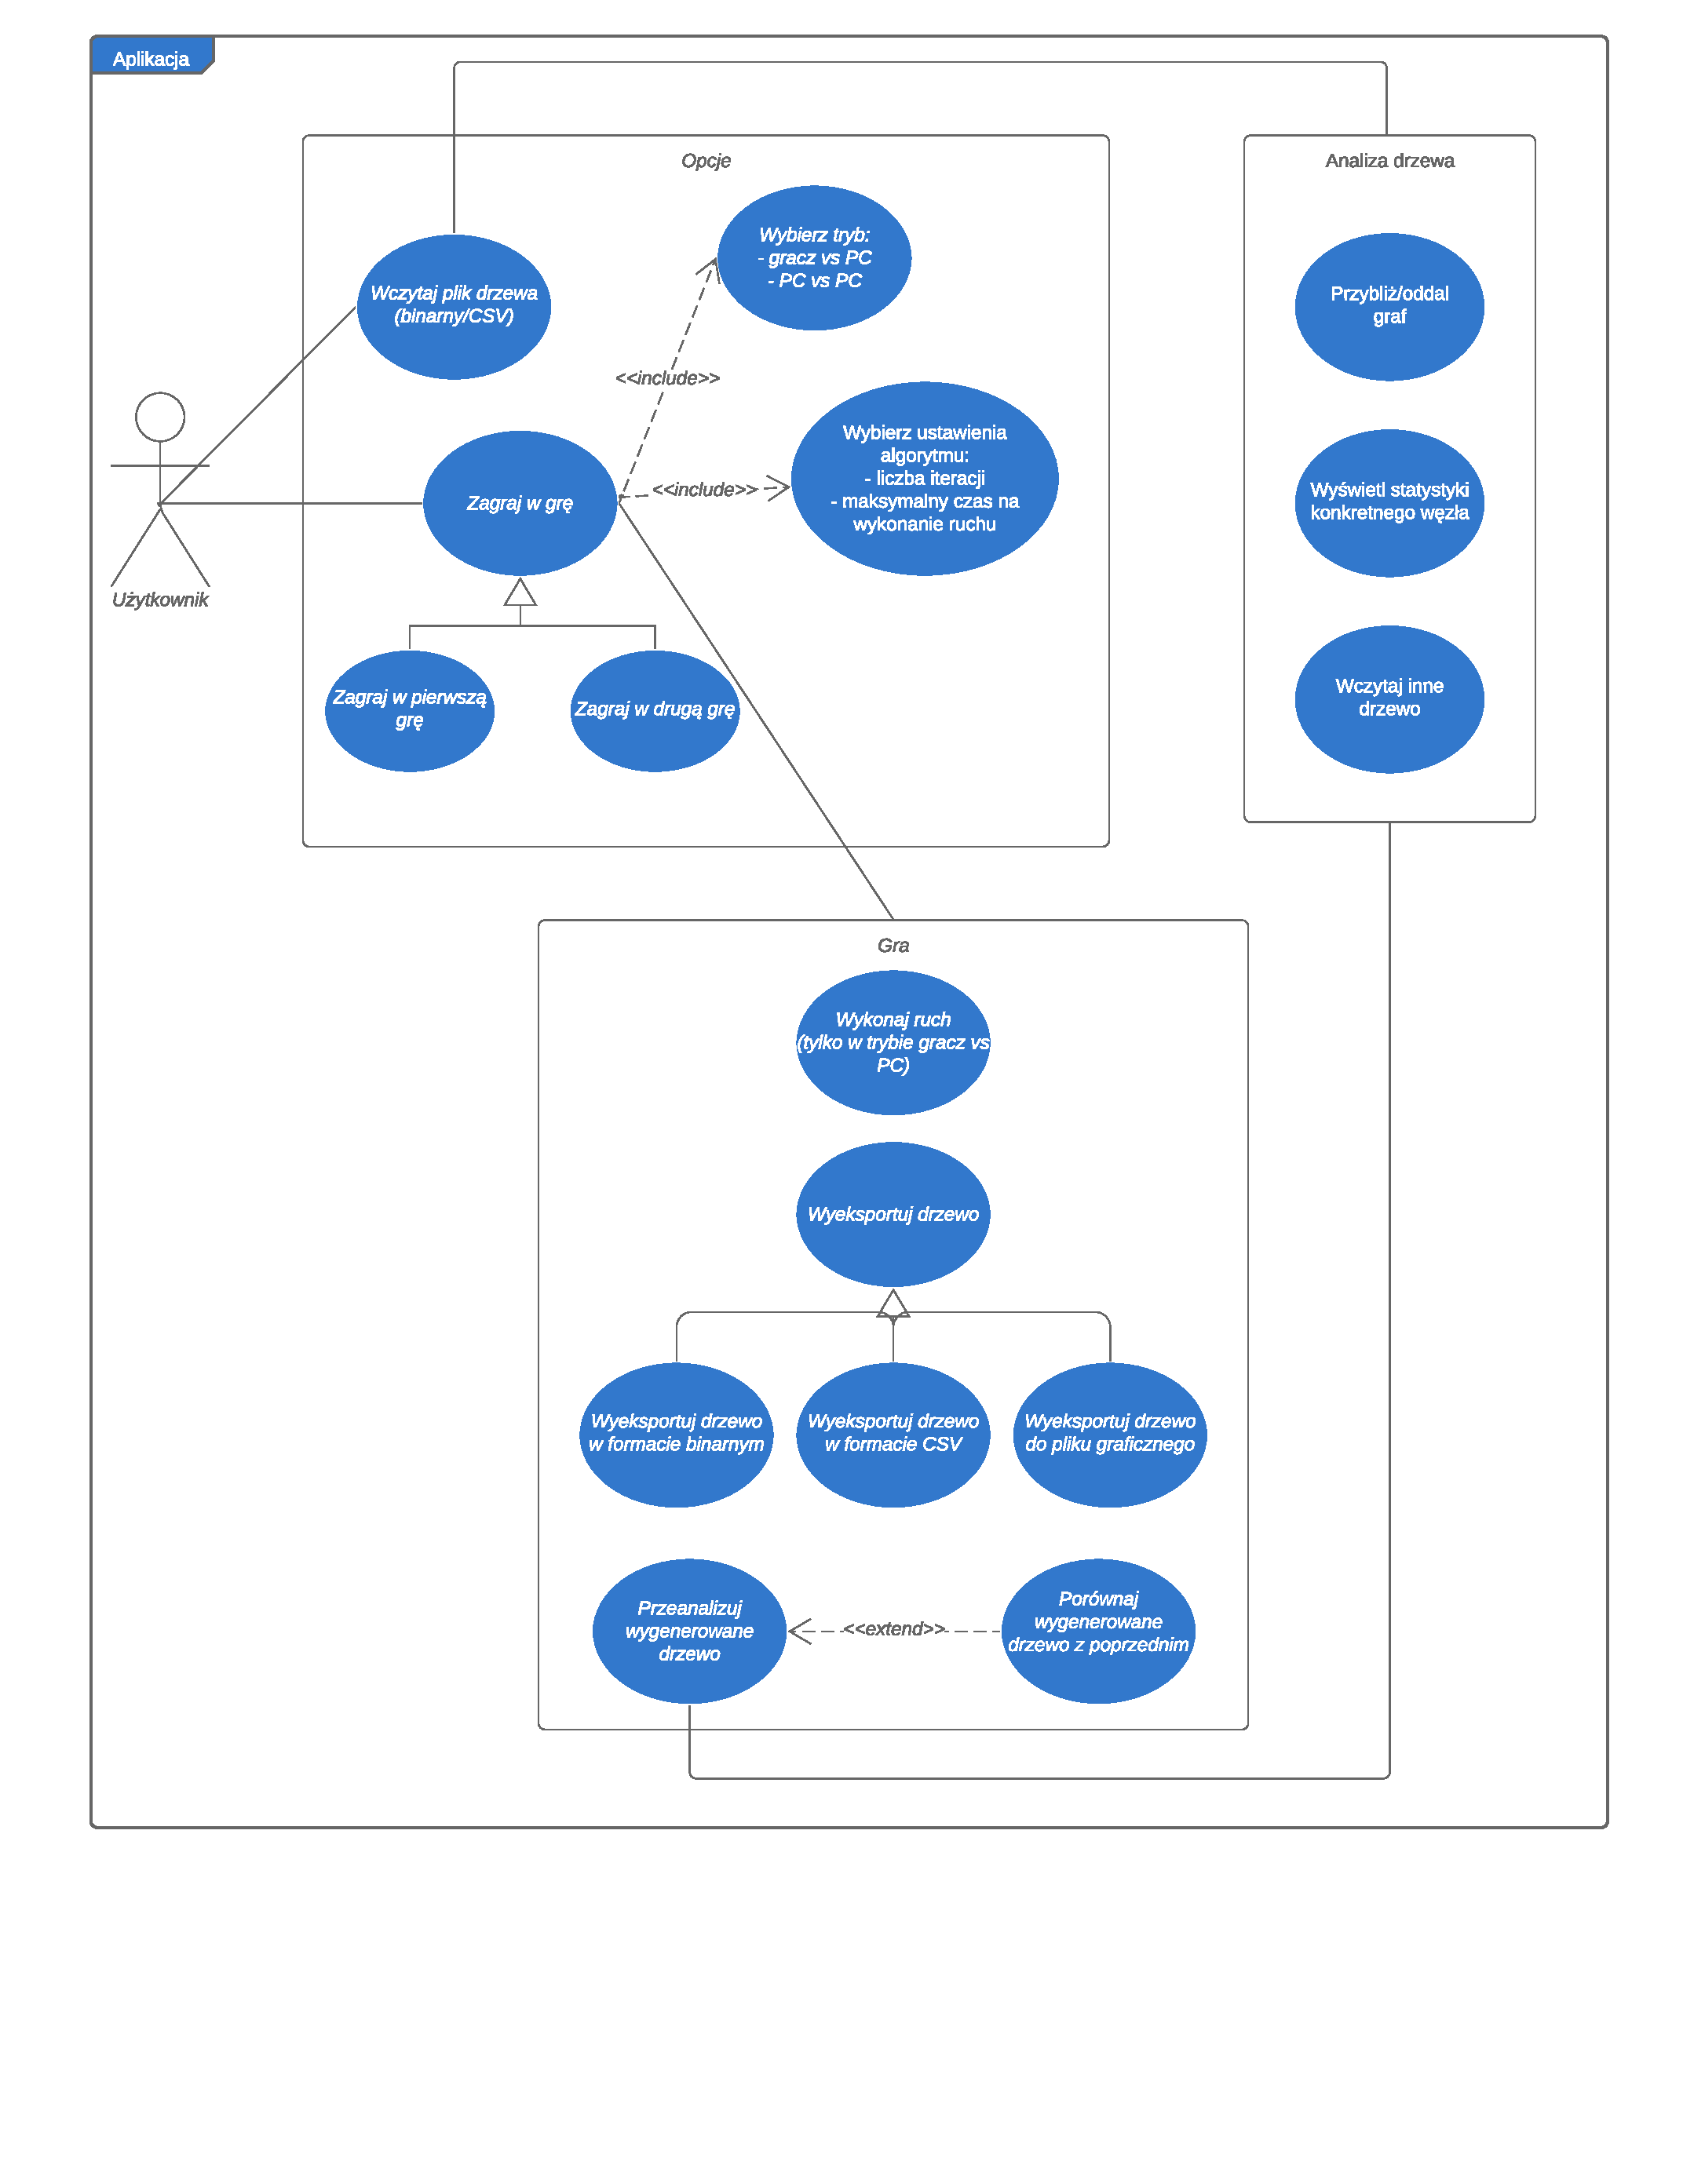
\includegraphics[width=\textwidth, trim={0 6.5cm 0 0},clip]{aplikacja-use-case-eps}
	\caption{Diagram przypadków użycia}
	\label{rys:usecase}
\end{figure}
\subsection{Założenia niefunkcjonalne}


% ------------------- 3. TEORIA ---------------------
\chapter{Teoria}
\section{Algorytmy MCTS}
\subsection{Opis grupy algorytmów}
\textbf{MCTS} (Monte Carlo Tree Search) - heurystyka podejmowania decyzji w pewnych zadaniach sztucznej inteligencji, np. ruchów w grach. Najczęściej MCTS opiera się na jakimś wariancie metody UCT.

\section{Algorytm UCT}
\textbf{UCT} (Upper Confidence Bound Applied to Trees) - algorytm przeszukujący drzewo stanów rozgrywki w poszukiwaniu najbardziej opłacalnych ruchów. Algorytm stara się zachować równowagę między eksploatacją ruchów po ruchach o wysokiej średniej wygranej a eksploracją tych mało sprawdzonych.
\subsection{Opis algorytmu}
\subsection{Dodatkowe założenia}
\section{Algorytm wizualizacji drzewa}
\subsection{Określenie problematyki}
\subsection{Usprawniony algorytm Walkera}


% ------------------- 4. IMPLEMENTACJA ---------------------
\chapter{Implementacja}
\section{Wykorzystane technologie}
\section{Architektura i działanie systemu}
\subsection{Moduły}
\subsection{Główne komponenty aplikacji}
\subsection{Interfejs użytkownika}


% ------------------- 5. INSTRUKCJE ---------------------
\chapter{Instrukcje}
\section{Instrukcja instalacji}
\section{Instrukcja użytkownika}


% ------------------- 6. OCENA I PODSUMOWANIE---------------------
\chapter{Podsumowanie i ocena}
\section{Uzyskane efekty}
\section{Kontynuacja pracy}
\section{Wydajność}
\section{Testy akceptacyjne}


% ------------------- 6. WNIOSKI ---------------------
\chapter{Wnioski}
